% AcademiX - Presentacion Entrega 2
% Compilar con pdfLaTeX.
% Objetivo: slides visuales, pocas palabras, anexos para preguntas.
\documentclass[aspectratio=169,10pt]{beamer}

\usetheme{Boadilla}
\usepackage[utf8]{inputenc}
\usepackage[T1]{fontenc}
\usepackage[spanish,es-noshorthands]{babel}
\usepackage{graphicx}
\usepackage{tabularx}
\usepackage{booktabs}
\usepackage{xcolor}
\usepackage{tikz}
\usepackage{array}

\usetikzlibrary{arrows.meta,positioning,fit,calc,shapes.geometric}

\definecolor{academixnavy}{HTML}{18324F}
\definecolor{academixblue}{HTML}{2563EB}
\definecolor{academixteal}{HTML}{0F766E}
\definecolor{academixamber}{HTML}{B7791F}
\definecolor{academixgreen}{HTML}{15803D}
\definecolor{academixred}{HTML}{B91C1C}
\definecolor{academixbg}{HTML}{F8FAFC}
\definecolor{academixsoftblue}{HTML}{EFF6FF}
\definecolor{academixsoftteal}{HTML}{F0FDFA}
\definecolor{academixsoftamber}{HTML}{FFFBEB}
\definecolor{academixline}{HTML}{CBD5E1}
\definecolor{academixslate}{HTML}{475569}
\definecolor{academixmuted}{HTML}{64748B}

\setbeamercolor{structure}{fg=academixnavy}
\setbeamercolor{frametitle}{fg=academixnavy,bg=academixbg}
\setbeamercolor{title}{fg=academixnavy}
\setbeamercolor{block title}{fg=white,bg=academixnavy}
\setbeamercolor{block body}{fg=black,bg=academixbg}
\setbeamercolor{alerted text}{fg=academixamber}
\setbeamertemplate{navigation symbols}{}
\setbeamertemplate{footline}[frame number]
\setbeamerfont{frametitle}{size=\large,series=\bfseries}
\setbeamerfont{title}{series=\bfseries}

\newcolumntype{Y}{>{\raggedright\arraybackslash}X}
\newcommand{\chip}[2]{\tikz[baseline=(n.base)]\node[rounded corners=2pt,fill=#1,inner xsep=5pt,inner ysep=2pt,text=white,font=\scriptsize\bfseries](n){#2};}
\newcommand{\softchip}[3]{\tikz[baseline=(n.base)]\node[rounded corners=2pt,draw=#1,fill=#2,inner xsep=5pt,inner ysep=2pt,text=#1,font=\scriptsize\bfseries](n){#3};}
\newcommand{\kpi}[3]{%
\begin{tikzpicture}
  \node[draw=#1,fill=#1!7,rounded corners=3pt,minimum width=0.28\textwidth,minimum height=1.15cm,align=center] {
    {\Large\bfseries\color{#1}#2}\\[-1pt]
    {\scriptsize #3}
  };
\end{tikzpicture}}

\title[AcademiX]{AcademiX}
\subtitle{Entrega 2: diseño preliminar, riesgos y walking skeleton}
\author[Equipo Lock In]{Equipo Lock In}
\institute[IIC3143]{IIC3143 Desarrollo de Software}
\date{Octubre 2026}

\begin{document}

\begin{frame}
  \titlepage
  \vspace{-0.25cm}
  \centering
  \softchip{academixnavy}{academixsoftblue}{Curso}
  \softchip{academixteal}{academixsoftteal}{Material}
  \softchip{academixamber}{academixsoftamber}{Quizzes}
  \softchip{academixgreen}{green!8}{Notas}
  \softchip{academixslate}{academixbg}{Auditoría}
\end{frame}

\begin{frame}{Qué se debía demostrar}
\begin{columns}[T,onlytextwidth]
\begin{column}{0.48\textwidth}
\begin{block}{Artefactos de diseño}
\small
\begin{itemize}
  \item Casos de uso actualizados.
  \item Arquitectura preliminar.
  \item Modelo de dominio.
  \item Modelo de datos.
\end{itemize}
\end{block}
\end{column}
\begin{column}{0.48\textwidth}
\begin{block}{Gestión y validación}
\small
\begin{itemize}
  \item Plan de desarrollo.
  \item Riesgos actualizados.
  \item Walking skeleton CI/CD.
  \item Evidencia de despliegue.
\end{itemize}
\end{block}
\end{column}
\end{columns}
\vspace{0.35cm}
\centering
\hspace*{0.18\textwidth}
\kpi{academixblue}{16}{casos de uso MVP}\hfill
\kpi{academixamber}{7}{semanas de ejecución}
\hspace*{0.18\textwidth}
\end{frame}

\begin{frame}{Alcance MVP}
\begin{columns}[T,onlytextwidth]
\begin{column}{0.48\textwidth}
\begin{block}{Docente}
\small
\begin{itemize}
  \item Crear cursos, secciones y roles.
  \item Organizar módulos y material.
  \item Crear quizzes autocorregidos.
  \item Configurar y publicar notas.
\end{itemize}
\end{block}
\end{column}
\begin{column}{0.48\textwidth}
\begin{block}{Estudiante}
\small
\begin{itemize}
  \item Elegir institución autorizada.
  \item Ver cursos y material publicado.
  \item Responder quizzes.
  \item Consultar notas y promedio.
\end{itemize}
\end{block}
\end{column}
\end{columns}
\vspace{0.25cm}
\centering
\softchip{academixred}{red!6}{Fuera: admin institucional}
\softchip{academixred}{red!6}{IA}
\softchip{academixred}{red!6}{chat}
\softchip{academixred}{red!6}{calendario}
\softchip{academixred}{red!6}{microservicios}
\end{frame}

\begin{frame}{Qué cambió frente a Entrega 1}
\begin{columns}[T,onlytextwidth]
\begin{column}{0.48\textwidth}
\begin{block}{Antes}
\small
\begin{itemize}
  \item GCP como destino principal.
  \item Base de datos por tenant.
  \item Tenant Registry.
  \item Pools por tenant.
  \item Workers/Redis condicionados.
\end{itemize}
\end{block}
\end{column}
\begin{column}{0.48\textwidth}
\begin{block}{Ahora}
\small
\begin{itemize}
  \item Railway como despliegue inmediato.
  \item PostgreSQL compartida.
  \item \texttt{institution\_id} como frontera lógica.
  \item PgBouncer compartido.
  \item HA y Bucket para operación.
\end{itemize}
\end{block}
\end{column}
\end{columns}
\vspace{0.2cm}
\begin{center}
\large\textbf{\color{academixnavy}Menos complejidad prematura, mismas garantías críticas.}
\end{center}
\end{frame}

\begin{frame}{Casos de uso por flujo}
\centering
\vspace{-0.1cm}
\begin{tikzpicture}[
  font=\sffamily\tiny,
  flow/.style={rounded corners=4pt,minimum width=2.65cm,minimum height=1.55cm,align=left,text width=2.45cm,inner sep=4pt},
  arrow/.style={-{Latex[length=2mm]},draw=academixnavy,thick}
]
\node[flow,draw=academixnavy,fill=academixnavy!8] (a) at (0,0) {\textbf{Acceso}\\CU-01 Institución\\CU-02 Contexto};
\node[flow,draw=academixteal,fill=academixteal!8] (b) at (3,0) {\textbf{Cursos}\\CU-03 Cursos visibles\\CU-04 Roles/secciones};
\node[flow,draw=academixblue,fill=academixblue!8] (c) at (6,0) {\textbf{Material}\\CU-05 Publicar\\CU-06 Consultar\\CU-14 Módulos};
\node[flow,draw=academixamber,fill=academixamber!8] (d) at (9,0) {\textbf{Quizzes}\\CU-07 Crear\\CU-08 Responder\\CU-09 Enviar\\CU-15 Cancelar};
\node[flow,draw=academixgreen,fill=academixgreen!8] (e) at (12,0) {\textbf{Notas}\\CU-10 Libro\\CU-11 Publicar\\CU-12 Ver\\CU-16 Revisar};
\node[flow,draw=academixslate,fill=academixslate!8] (f) at (6,-2.15) {\textbf{Auditoría}\\CU-13 Historial};
\draw[arrow] (a) -- (b);
\draw[arrow] (b) -- (c);
\draw[arrow] (c) -- (d);
\draw[arrow] (d) -- (e);
\draw[arrow] (e) |- (f);
\draw[arrow] (f) -| (b);
\end{tikzpicture}
\vspace{0.3cm}

\small El flujo prioriza el ciclo académico crítico: institución, curso, material, evaluación, nota y trazabilidad.
\end{frame}

\begin{frame}{RNF clave}
\centering
\begin{tikzpicture}[
  font=\sffamily\small,
  tile/.style={rounded corners=5pt,minimum width=3.05cm,minimum height=1.35cm,align=center,text width=2.7cm},
]
\node[tile,draw=academixnavy,fill=academixnavy!8] at (0,1.5) {\textbf{Aislamiento}\\Institution + scope};
\node[tile,draw=academixblue,fill=academixblue!8] at (3.4,1.5) {\textbf{Seguridad}\\JWT + membership};
\node[tile,draw=academixgreen,fill=academixgreen!8] at (6.8,1.5) {\textbf{Integridad}\\FK + constraints};
\node[tile,draw=academixamber,fill=academixamber!8] at (1.7,0) {\textbf{Auditoría}\\cambios sensibles};
\node[tile,draw=academixteal,fill=academixteal!8] at (5.1,0) {\textbf{Operación}\\Docker + CI/CD + HA};
\end{tikzpicture}
\vspace{0.45cm}

\begin{block}{Decisión}
\small Las garantías importantes viven en autorización, modelo de datos, trazabilidad y despliegue reproducible.
\end{block}
\end{frame}

\begin{frame}{Arquitectura objetivo}
\centering
\resizebox{0.95\textwidth}{!}{%
\begin{tikzpicture}[
  font=\sffamily\footnotesize,
  base/.style={draw=academixnavy,thick,fill=academixsoftblue,rounded corners=3pt,align=center,inner sep=4pt,text width=2.6cm},
  ops/.style={draw=academixteal,thick,fill=academixsoftteal,rounded corners=3pt,align=center,inner sep=4pt,text width=2.6cm},
  data/.style={draw=academixamber,thick,fill=academixsoftamber,rounded corners=3pt,align=center,inner sep=4pt,text width=2.8cm},
  tenant/.style={draw=academixslate,thick,fill=white,rounded corners=2pt,align=center,inner sep=3pt,text width=2.2cm},
  fl/.style={-{Latex[length=1.8mm]},draw=academixnavy,thick},
  repl/.style={-{Latex[length=1.8mm]},draw=academixamber,thick,dashed}
]
\node[base] (u) at (0,0) {\textbf{Usuarios}\\docente · estudiante\\ayudante};
\node[ops] (edge) at (3.4,0) {\textbf{Railway edge}\\load balancing};
\node[base] (fe) at (6.8,0.9) {\textbf{Next.js}\\frontend réplicas};
\node[base] (be) at (6.8,-0.9) {\textbf{NestJS}\\backend réplicas\\stateless};
\node[ops] (pool) at (10.2,-0.9) {\textbf{PgBouncer}\\connection pool};
\node[ops] (hap) at (13.6,-0.9) {\textbf{HAProxy}\\PostgreSQL HA};
\node[data] (dbp) at (17.0,-0.25) {\textbf{Primary}\\schema compartido};
\node[data] (dbr) at (17.0,-1.75) {\textbf{Replica}\\failover};
\node[data] (bucket) at (10.2,-3.0) {\textbf{Railway Bucket}\\PDF · presentaciones\\adjuntos};
\node[tenant] (uc) at (14.0,1.65) {Institution UC};
\node[tenant] (utfsm) at (16.8,1.65) {Institution UTFSM};
\node[tenant] (other) at (19.6,1.65) {Institution ...};
\coordinate (split) at (17.0,0.85);

\draw[fl] (u) -- (edge);
\draw[fl] (edge) -- (fe);
\draw[fl] (edge) -- (be);
\draw[fl] (fe) -- (be);
\draw[fl] (be) -- (pool);
\draw[fl] (pool) -- (hap);
\draw[fl] (hap) -- (dbp);
\draw[repl] (dbp) -- node[right,font=\scriptsize]{streaming} (dbr);
\draw[fl] (be) |- (bucket);
\draw[fl] (dbp.north) -- (split);
\draw[fl] (split) -| (uc.south);
\draw[fl] (split) -- (utfsm.south);
\draw[fl] (split) -| (other.south);
\node[align=left,font=\sffamily\scriptsize] at (3.5,-3.05) {%
\textcolor{academixnavy}{\rule{0.32cm}{0.6pt}} base del despliegue\\
\textcolor{academixamber}{\rule{0.32cm}{0.6pt}} disponibilidad/failover\\
\textbf{HA:} High Availability\\
\textbf{Tenant lógico:} \texttt{institution\_id} + autorización + FK};
\end{tikzpicture}}
\end{frame}

\begin{frame}{Preguntas de falla}
\small
\begin{tabularx}{\textwidth}{lYY}
\toprule
\textbf{Si cae...} & \textbf{Respuesta} & \textbf{Límite} \\
\midrule
Frontend/backend réplica & Railway envía tráfico a réplicas sanas. & Requiere más de una réplica. \\
Backend completo & Healthcheck y restart policy. & Si es bug, rollback o fix. \\
PgBouncer & Se pierde endpoint pooleado. & Escalar réplicas y conservar URL no pooleada. \\
Primary DB & Patroni promueve réplica; HAProxy redirige. & Conexiones en vuelo deben reintentar. \\
Datos corruptos & Backups y PITR. & HA también propaga errores lógicos. \\
Object storage & Core sin archivos puede seguir. & Cargas/descargas fallan temporalmente. \\
Proveedor/región & Riesgo aceptado MVP. & No hay multi-cloud. \\
\bottomrule
\end{tabularx}
\end{frame}

\begin{frame}{Multi-tenancy lógico}
\centering
\vspace{-0.1cm}
\resizebox{0.92\textwidth}{!}{%
\begin{tikzpicture}[
  font=\sffamily\scriptsize,
  box/.style={rounded corners=3pt,minimum width=3cm,minimum height=0.85cm,align=center,inner sep=3pt},
  wide/.style={rounded corners=3pt,minimum width=4cm,minimum height=0.9cm,align=center,inner sep=3pt},
  arr/.style={-{Latex[length=1.7mm]},draw=academixnavy,thick},
  scope/.style={draw=academixslate,dashed,rounded corners=5pt,inner sep=8pt}
]
\node[box,draw=academixnavy,fill=academixnavy!7] (user) at (0,2.75) {\textbf{User}\\global};
\node[box,draw=academixteal,fill=academixteal!7] (mem) at (4.0,2.75) {\textbf{InstitutionMembership}\\acceso institucional};
\node[box,draw=academixamber,fill=academixamber!8] (inst) at (8.0,2.75) {\textbf{Institution}\\tenant lógico};

\node[box,draw=academixblue,fill=academixblue!7] (course) at (8.0,1.3) {\textbf{Course}\\curso};
\node[box,draw=academixblue,fill=academixblue!7] (section) at (4.0,1.3) {\textbf{Section}\\sala lógica};
\node[box,draw=academixgreen,fill=academixgreen!7] (enroll) at (0,1.3) {\textbf{Enrollment}\\rol académico};

\node[wide,draw=academixslate,fill=white] (owned) at (8.0,-0.25) {\textbf{Tenant-owned}\\Material · Quiz · Grade · AuditEvent};

\node[wide,draw=academixnavy,fill=academixsoftblue,text width=4.2cm] (rule) at (12.5,1.6) {\textbf{Regla central}\\El path selecciona contexto;\\no autentica ni autoriza.};
\node[wide,draw=academixteal,fill=academixsoftteal,text width=4.2cm] (guard) at (12.5,0.1) {\textbf{Defensa}\\membership + enrollment +\\\texttt{institution\_id} + FK};

\draw[arr] (user) -- (mem);
\draw[arr] (mem) -- (inst);
\draw[arr] (inst) -- (course);
\draw[arr] (course) -- (section);
\draw[arr] (section) -- (enroll);
\draw[arr] (user) -- (enroll);
\draw[arr] (course) -- (owned);
\draw[arr] (inst) -- (rule);
\draw[arr] (owned.east) -- (guard.west);
\end{tikzpicture}}
\vspace{0.2cm}

\small \texttt{Enrollment} une usuario, institución, curso, sección y rol; las entidades académicas se filtran y validan por \texttt{institution\_id}.
\end{frame}

\begin{frame}{Modelo de dominio}
\centering
\vspace{-0.1cm}
\resizebox{0.95\textwidth}{!}{%
\begin{tikzpicture}[
  font=\sffamily\scriptsize,
  entity/.style={draw=academixnavy,fill=academixbg,rounded corners=3pt,minimum width=2.45cm,minimum height=0.8cm,align=center},
  core/.style={draw=academixteal,fill=academixsoftteal,rounded corners=3pt,minimum width=2.45cm,minimum height=0.8cm,align=center},
  grade/.style={draw=academixamber,fill=academixsoftamber,rounded corners=3pt,minimum width=2.45cm,minimum height=0.8cm,align=center},
  arr/.style={-{Latex[length=1.5mm]},draw=academixslate,thick}
]
\node[entity] (u) at (0,1.6) {User};
\node[entity] (im) at (3.4,1.6) {InstitutionMembership};
\node[entity] (i) at (6.8,1.6) {Institution};
\node[core] (c) at (10.2,1.6) {Course};
\node[core] (s) at (13.6,1.6) {Section};
\node[core] (e) at (13.6,0.25) {Enrollment};

\node[core] (m) at (10.2,-1.1) {CourseModule};
\node[core] (mat) at (6.8,-1.1) {Material};
\node[grade] (q) at (13.6,-1.1) {Quiz};
\node[grade] (qa) at (17.0,-1.1) {QuizAttempt};

\node[grade] (gi) at (10.2,-2.45) {GradeItem};
\node[grade] (g) at (13.6,-2.45) {Grade};
\node[entity] (a) at (17.0,-2.45) {AuditEvent};

\draw[arr] (u) -- (im);
\draw[arr] (im) -- (i);
\draw[arr] (i) -- (c);
\draw[arr] (c) -- (s);
\draw[arr] (s) -- (e);
\draw[arr] (c) -- (m);
\draw[arr] (m) -- (mat);
\draw[arr] (m) -- (q);
\draw[arr] (q) -- (qa);
\draw[arr] (q.south) -- ++(0,-0.38) -| (gi.north);
\draw[arr] (gi) -- (g);
\draw[arr] (g) -- (a);
\end{tikzpicture}}
\vspace{0.15cm}

\small Dominio acotado: no hay coordinador ni RBAC completo; docente con rol \texttt{teacher} administra su curso/secciones.
\end{frame}

\begin{frame}{Modelo de datos}
\scriptsize
\begin{tabularx}{\textwidth}{p{2.1cm}p{3.5cm}Y}
\toprule
\textbf{Categoría} & \textbf{Tabla} & \textbf{Descripción} \\
\midrule
Global & \texttt{institutions} & Tenant lógico: slug, nombre, estado y ciclo de vida. \\
Global & \texttt{users} & Identidad global reutilizable entre instituciones. \\
Acceso & \texttt{institution\_memberships} & Habilita acceso de usuario a institución. \\
Curso & \texttt{courses}, \texttt{sections} & Curso semestral y separación lógica por sección. \\
Curso & \texttt{enrollments} & Une usuario, institución, curso, sección y rol académico. \\
Contenido & \texttt{course\_modules}, \texttt{materials} & Organización del material común visible para secciones del curso. \\
Evaluación & \texttt{quizzes}, \texttt{quiz\_attempts} & Quiz con preguntas JSONB e intentos estudiantiles. \\
Notas & \texttt{grade\_items}, \texttt{grades} & Columnas del libro y notas concretas por estudiante. \\
Auditoría & \texttt{audit\_events} & Historial inmutable de cambios sensibles. \\
\bottomrule
\end{tabularx}
\vspace{0.2cm}

\small Catálogo completo adjunto en XLSX/CSV con columnas, tipos, PK/FK, nulabilidad y descripciones.
\end{frame}

\begin{frame}{Walking skeleton y evidencia}
\begin{columns}[T,onlytextwidth]
\begin{column}{0.32\textwidth}
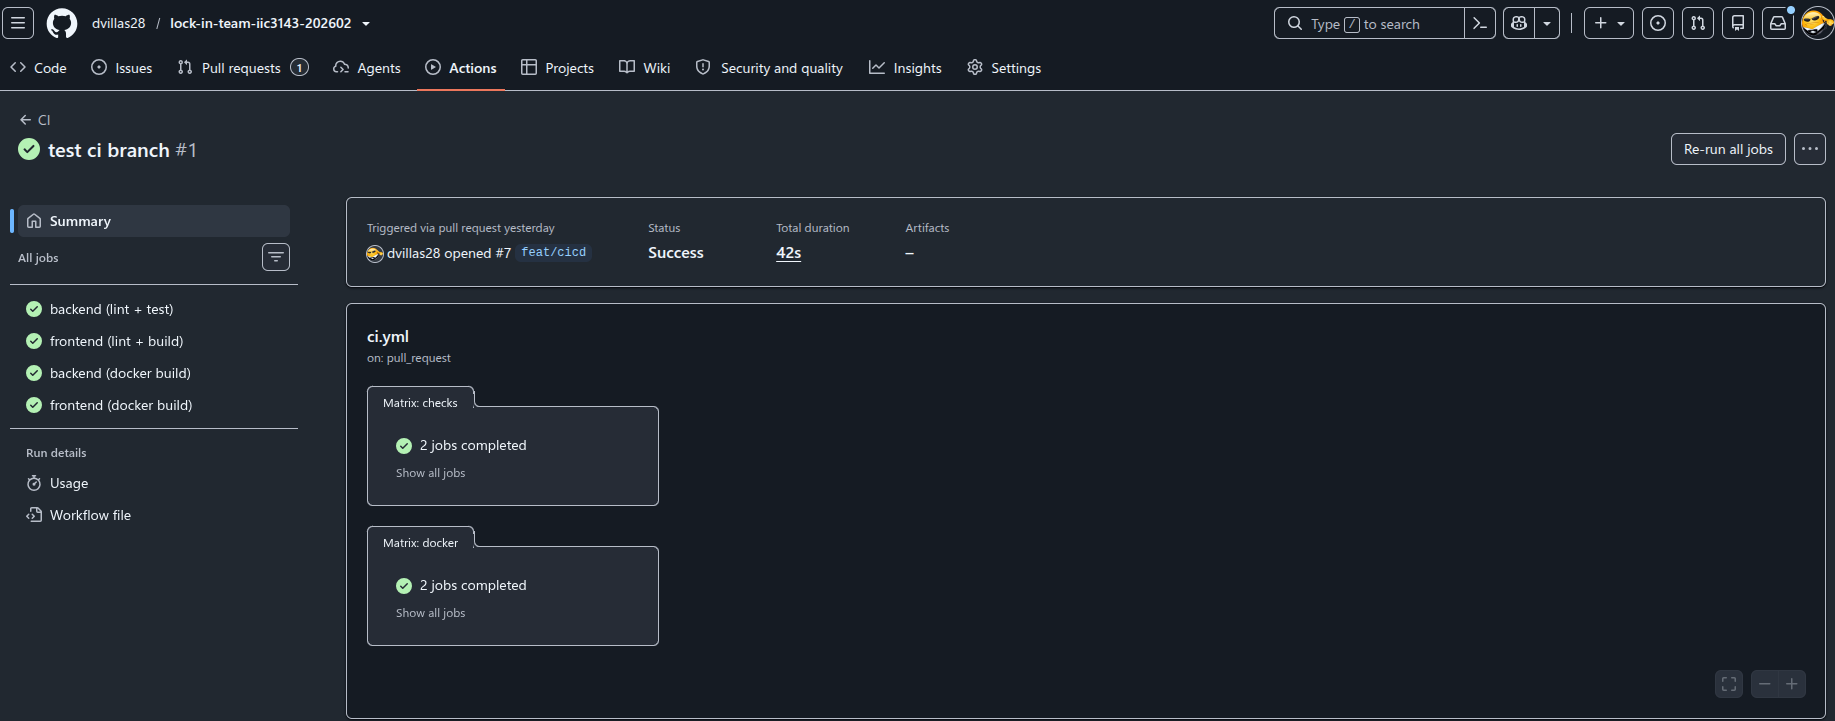
\includegraphics[width=\textwidth,height=0.48\textheight,keepaspectratio]{../11-cicd-evidence/img/03-ci-run.png}
\centering\scriptsize CI ejecutado
\end{column}
\begin{column}{0.32\textwidth}
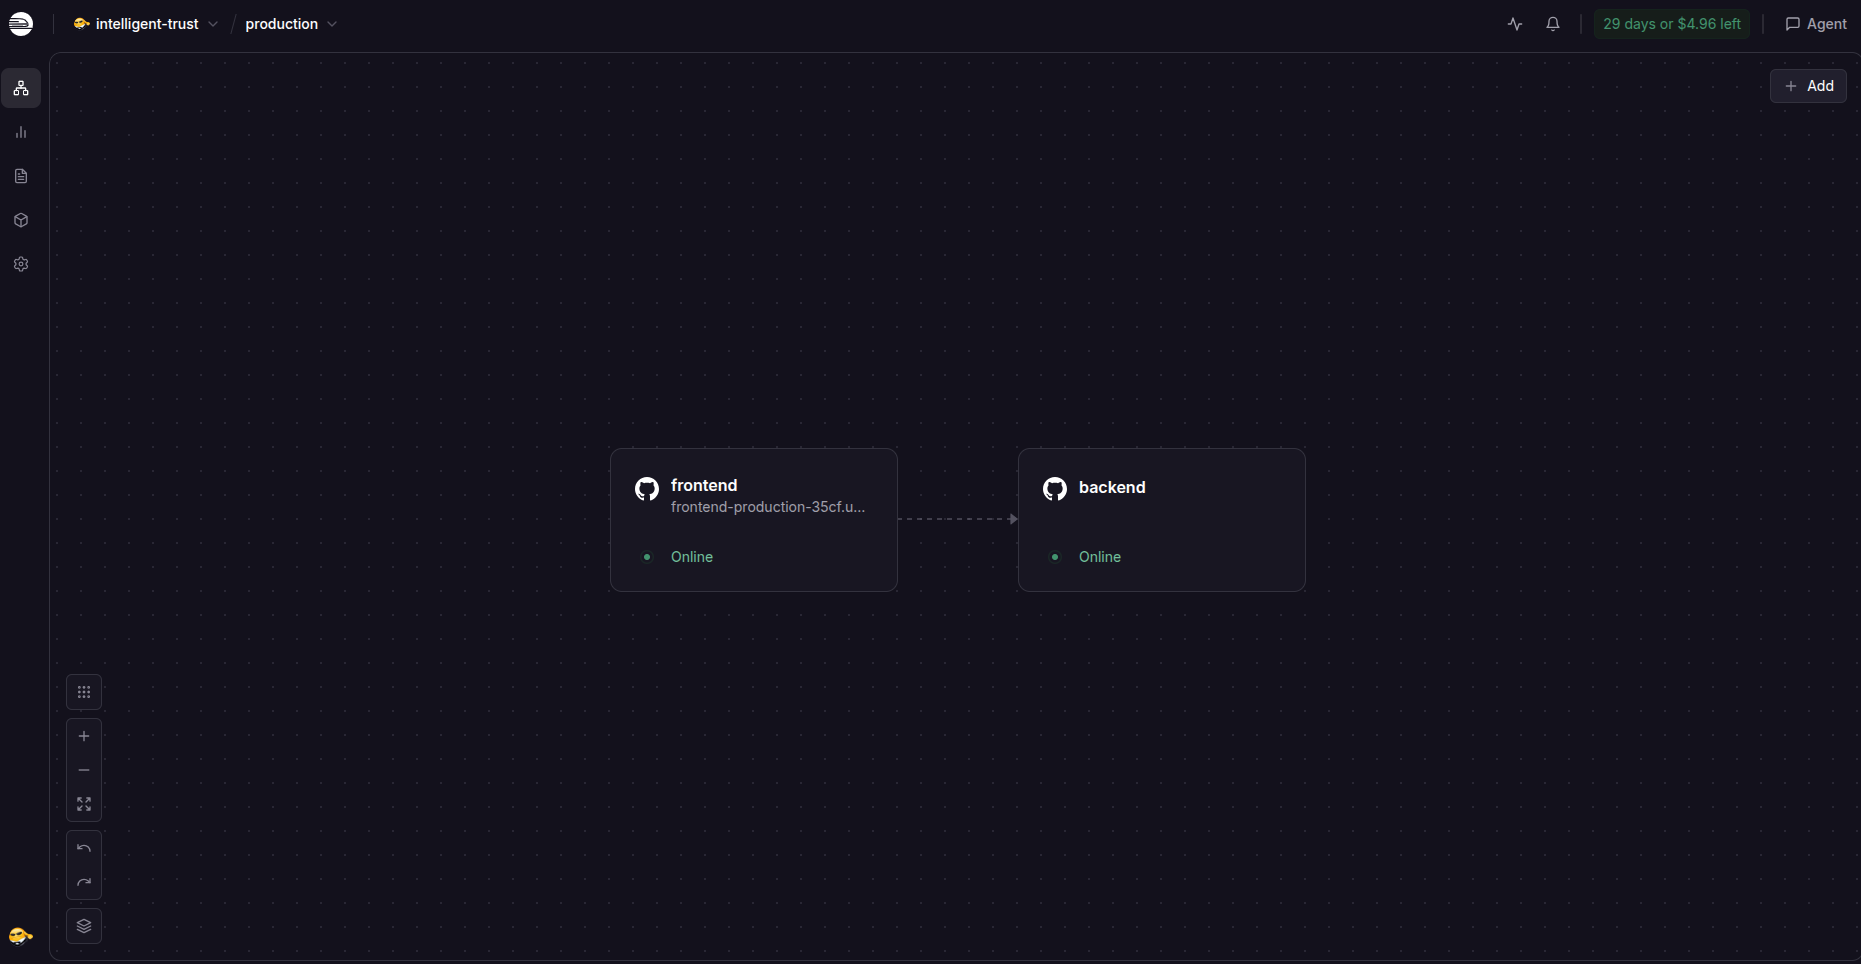
\includegraphics[width=\textwidth,height=0.48\textheight,keepaspectratio]{../11-cicd-evidence/img/06-railway-project.png}
\centering\scriptsize Railway
\end{column}
\begin{column}{0.32\textwidth}
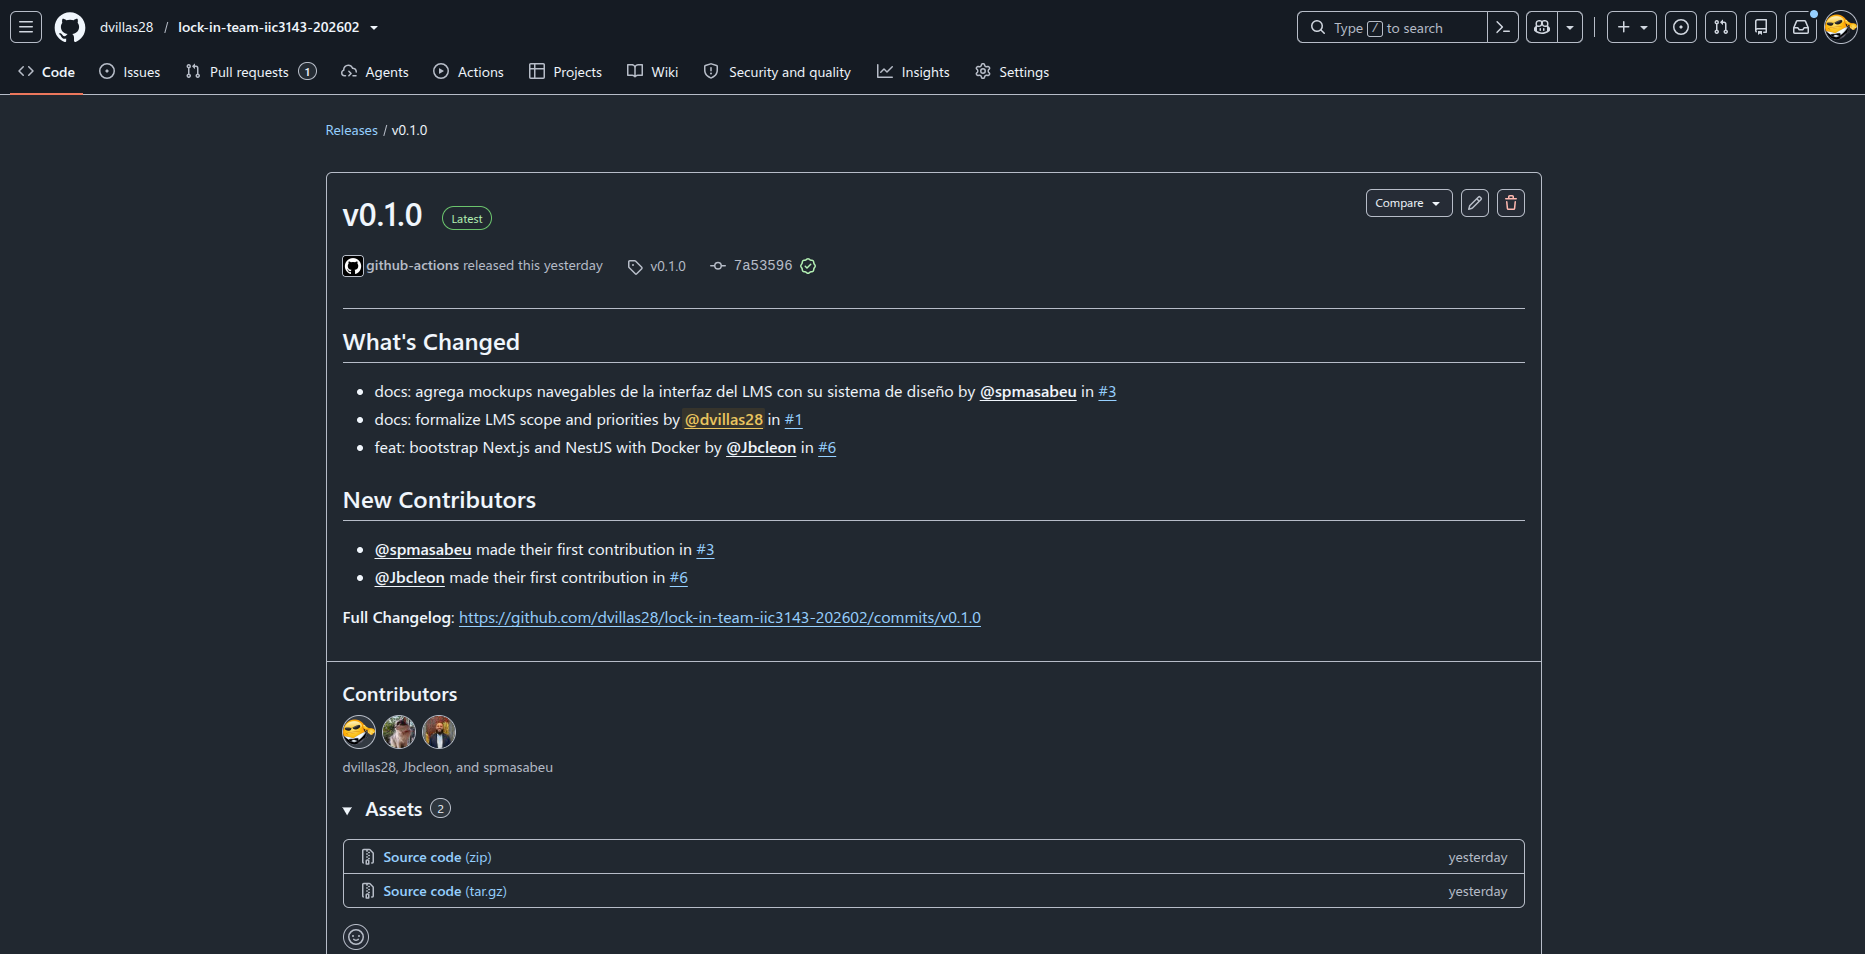
\includegraphics[width=\textwidth,height=0.48\textheight,keepaspectratio]{../11-cicd-evidence/img/11-github-release.png}
\centering\scriptsize Release
\end{column}
\end{columns}
\vspace{0.25cm}
\begin{block}{Riesgo mitigado}
\small Integración frontend/backend, Docker, CI, despliegue Railway y release por tag.
\end{block}
\end{frame}

\begin{frame}{Plan de desarrollo: 7 semanas}
\centering
\resizebox{\textwidth}{!}{%
\begin{tikzpicture}[
  font=\sffamily\scriptsize,
  week/.style={rounded corners=3pt,minimum width=2.35cm,minimum height=1.15cm,align=center,text width=2.15cm},
  arr/.style={-{Latex[length=1.8mm]},draw=academixnavy,thick}
]
\node[week,draw=academixnavy,fill=academixnavy!8] (w1) at (0,0) {\textbf{1}\\Plan + CI/CD\\05 oct};
\node[week,draw=academixteal,fill=academixteal!8] (w2) at (2.7,0) {\textbf{2}\\DB + identidad};
\node[week,draw=academixblue,fill=academixblue!8] (w3) at (5.4,0) {\textbf{3}\\Aislamiento};
\node[week,draw=academixgreen,fill=academixgreen!8] (w4) at (8.1,0) {\textbf{4}\\Cursos + UI shell};
\node[week,draw=academixamber,fill=academixamber!8] (w5) at (10.8,0) {\textbf{5}\\Material + quizzes};
\node[week,draw=academixred,fill=academixred!8] (w6) at (13.5,0) {\textbf{6}\\Notas + auditoría};
\node[week,draw=academixslate,fill=academixslate!8] (w7) at (16.2,0) {\textbf{7}\\Hardening\\22 nov};
\draw[arr] (w1) -- (w2);
\draw[arr] (w2) -- (w3);
\draw[arr] (w3) -- (w4);
\draw[arr] (w4) -- (w5);
\draw[arr] (w5) -- (w6);
\draw[arr] (w6) -- (w7);
\end{tikzpicture}}
\vspace{0.3cm}

\small Responsables: Fierro bot PR reviewer · Palma backend/infra · Contreras/Matías frontend · Villaseñor CI/CD y gestión.
\end{frame}

\begin{frame}{Riesgos principales}
\centering
\begin{tikzpicture}[
  font=\sffamily\scriptsize,
  risk/.style={rounded corners=3pt,align=center,text width=2.55cm,minimum height=0.85cm}
]
\draw[->,thick,academixslate] (0,0) -- (8.2,0) node[right]{Impacto};
\draw[->,thick,academixslate] (0,0) -- (0,5.0) node[above]{Probabilidad};
\draw[academixline] (4.0,0) -- (4.0,4.6);
\draw[academixline] (0,2.3) -- (8.0,2.3);
\node[risk,draw=academixred,fill=academixred!8] at (6.2,3.7) {R-01/R-02\\fuga o query sin scope};
\node[risk,draw=academixred,fill=academixred!8] at (2.0,3.7) {R-12\\sobrealcance};
\node[risk,draw=academixamber,fill=academixamber!8] at (6.2,1.4) {R-13\\auditoría incompleta};
\node[risk,draw=academixamber,fill=academixamber!8] at (2.0,1.4) {R-16\\bot reviewer ruidoso};
\node[font=\sffamily\scriptsize\bfseries,academixmuted] at (1.0,4.75) {alta};
\node[font=\sffamily\scriptsize\bfseries,academixmuted] at (7.3,0.35) {alto};
\end{tikzpicture}
\vspace{0.2cm}

\small Cada riesgo tiene responsable, mitigación y contingencia en la planilla completa.
\end{frame}

\begin{frame}{Cierre}
\centering
\begin{tikzpicture}[
  font=\sffamily\small,
  msg/.style={rounded corners=6pt,minimum width=3.8cm,minimum height=1.6cm,align=center,text width=3.3cm}
]
\node[msg,draw=academixnavy,fill=academixnavy!8] at (0,0) {\textbf{Diseño estable}\\MVP acotado y trazable};
\node[msg,draw=academixteal,fill=academixteal!8] at (4.4,0) {\textbf{Arquitectura defendible}\\HA, pooling, storage y fallas};
\node[msg,draw=academixamber,fill=academixamber!8] at (8.8,0) {\textbf{Ejecución lista}\\7 semanas, dueños y riesgos};
\end{tikzpicture}
\vspace{0.5cm}

\Large\textbf{\color{academixnavy}La siguiente fase es implementar, no rediseñar.}
\end{frame}

\appendix

\begin{frame}{Anexo: responsables}
\small
\begin{tabularx}{\textwidth}{lY}
\toprule
\textbf{Área} & \textbf{Responsable y alcance} \\
\midrule
Bot PR reviewer & Daniel Fierro: integración, reglas y evidencia. \\
Backend e infraestructura & Sebastián Palma: API, persistencia, aislamiento, Docker y Railway. \\
Frontend & Julián Contreras y Matías: vistas, consumo API, cursos, quizzes y notas. \\
CI/CD y gestión & Daniel Villaseñor: pipelines, releases, Scrum, planillas y presentación. \\
\bottomrule
\end{tabularx}
\end{frame}

\begin{frame}{Anexo: paquetes documentales}
\small
\begin{tabularx}{\textwidth}{lY}
\toprule
\textbf{Doc} & \textbf{Contenido} \\
\midrule
03 & Casos de uso y requerimientos. \\
04 & Arquitectura, fallas y decisiones frente a Entrega 1. \\
05 & Modelo de dominio y UML. \\
06 & Modelo de datos, constraints y ERD. \\
07 & Riesgos actualizados. \\
08 & Plan de trabajo de 7 semanas. \\
11 & Evidencia CI/CD y Railway. \\
13 & Catálogo de datos XLSX/CSV. \\
\bottomrule
\end{tabularx}
\end{frame}

\end{document}
